\documentclass[a4paper,10pt,french]{book}
\usepackage[margin=2cm]{geometry}
\usepackage[thinfonts]{uglix2}
\usepackage{ulem}
\setminted{fontsize=\small}\nouveaustyle
\begin{document}
\titre{Corrigé du DS2}{NSI2}{11/2021}


\section*{Bases de données}
\exo\\

Afin de lancer un nouveau service de streaming de musique, vous devez construire une base de données pour les morceaux de votre catalogue. Pour l’instant vous disposez d’une seule table avec les informations des morceaux. Voici \textbf{un extrait} de cette table :

\begin{center}
    \footnotesize
    \begin{tabular}{|c|c|c|c|c|c|c|}
        \hline
        \rowcolor{UGLiOrange} \color{white}\textbf{Titre} &\color{white}\textbf{Durée}&\color{white}\textbf{Artiste}	&\color{white}\textbf{Album}&\color{white}\textbf{Piste}&\color{white}\textbf{CD}	& \color{white}\textbf{Année}\\
        \hline
        Astronomy			&384	&Blue Öyster Cult 							&Secret Treaties		&8	&1	&1974\\
        \hline
        Stone Cold Crazy	&136	&Queen										&Sheer Heart attack		&8	&1	&1974\\
        \hline
        Under Pressure		&242 	&Queen and David Bowie						&Hot Space				&11	&2	&1982\\
        \hline
        The Outlaw Torn 	&589 	&Metallica									&Load					&14	&1	&1996\\
        \hline
        Fuel				&270 	&Metallica									&Reload					&1	&1	&1997\\
        \hline
        The Memory Remains	&279 	&Metallica and Marianne Faithfull			&Reload					&2	&1	&1997\\
        \hline
        Astronomy			&398 	&Metallica									&Garage Inc.			&8	&1	&1998\\
        \hline
        Stone Cold Crazy	&139	&Metallica									&Garage Inc.			&11	&2	&1998\\
        \hline
        Fuel				&276 	&Metallica and the San Francisco Symphony	&S\&M					&6	&1	&1999\\
        \hline
        The Outlaw Torn		&599	&Metallica and the San Francisco Symphony	&S\&M 					&6	&2	&1999\\
        \hline
    \end{tabular}			
\end{center}			

Cette table ne convient pas vraiment pour faire une base de données.

\textbf{1.} Expliquer pourquoi aucune des colonnes ne peut pas servir de clef primaire.
\begin{encadre}[Réponse]
    Dans chaque colonne, une valeur peut apparaître plusieurs fois : il peut y avoir plusieurs morceaux avec le même titre, la même durée, le même groupe \textit{et c\ae tera}.
\end{encadre}

\textbf{2.} Pourquoi est-ce que cette table est problématique si on veut rajouter des informations sur les artistes, comme leur nationalité?
\begin{encadre}[Réponse]
    Il peut y avoir plusieurs artistes, de nationalités différentes au sein d'un même morceau.
\end{encadre}

\textbf{3.} Quel est le problème si on souhaite chercher les morceaux d’un artiste ? Vous pourrez prendre l’exemple de Metallica.	
\begin{encadre}[Réponse]
    De même que précédemment, un artiste peut être associé à d'autres artistes. On pourrait imaginer une recherche avec un \mintinline{SQL}{WHERE ... LIKE '%Metallica%'} mais on
        risque de sélectionner d'autres artistes (on pourrait imaginer un groupe dénommé \og We Are Not Metallica\fg{}). 
    \end{encadre}
    
    Un ami vous suggère d'utiliser le schéma suivant :\\
    
    \textbf{Morceau}(\uline{titre\_id}, titre, duree, \dashuline{artiste\_id}, album, piste, cd, annee)\\
    \textbf{Artiste}(\uline{artiste\_id}, nom)\\
    
    \textbf{4.}	Expliquer pourquoi cette représentation ne permet toujours pas de gérer les morceaux fait par deux artistes différents.	
    
    \begin{encadre}[Réponse]
        Un titre est identifié de manière unique par \texttt{titre\_id} et associé à un unique \texttt{artiste\_id} : impossible de rajouter un autre artiste en gardant la même clé primaire.
    \end{encadre}
    Finalement, vous arrivez au schéma suivant :
    \begin{center}
        \includegraphics[width=12cm]{img/schema}
    \end{center}
    
    \textbf{5.}	Compléter les tables à l’aide des informations déjà disponibles. Un des morceaux n’a pas été intégré, inutile de l'y remettre. Si les noms dépassent, mettre uniquement le début.
    
    \begin{center}
        \begin{tabular}{|c|c|c|}
            \hline
            \rowcolor{UGLiOrange} \color{white}\textbf{titre\_id} &\color{white}\textbf{titre}&\color{white}\textbf{duree}\\
            \hline
            519 & Astronomy			&\color{red}384 \\
            \hline
            1219 &Astronomy	&\color{red}398 \\
            \hline
            316 & Stone Cold Crazy & 136\\
            \hline
            1319 & Stone Cold Crazy & 139\\
            \hline
            1298	&	\color{red}Fuel		&270\\
            \hline
            1570& \color{red}Fuel& \\
            \hline
            401 & \color{red}Under Pressure& \\
            \hline
            1125 & The Outlaw Torn& 589 \\
            \hline
            599 & The Outlaw Torn &599\\
            \hline
        \end{tabular}\hspace*{2em}
        \begin{tabular}{|c|c|}
            \hline
            \rowcolor{UGLiOrange} \color{white}\textbf{titre\_id} &\color{white}\textbf{artiste\_id}\\
            \hline
            519 & 25		\\
            \hline
            1219 &154	 \\
            \hline
            1319 &\color{red}154 \\
            \hline
            1298 & 154\\
            \hline
            1570	&154\\
            \hline
            1570&  318\\
            \hline
            1125 & 154 \\
            \hline
            1591 & 154\\
            \hline
            1591 & 318\\
            \hline
            316 & 79\\
            \hline
            401 & 79\\
            \hline
            401 & 108\\
            \hline
        \end{tabular}	\hspace*{2em}
        \begin{tabular}{|c|c|}
            \hline
            \rowcolor{UGLiOrange} \color{white}\textbf{artiste\_id} &\color{white}\textbf{nom}\\
            \hline
            \color{red} 154   & Metallica	\\
            \hline
            318& \color{red}San Francisco S. \\
            \hline
            25 & \color{red}Blue Öyster Cult\\
            \hline
            79 &\color{red} Queen \\
            \hline
            108	&\color{red} David Bowie\\
            \hline
        \end{tabular}
    \end{center}
    \textbf{6.} Comment appelle-t-on les clefs primaires de certaines tables apparaissant dans certaines tables, comme dans Interprete?
    \begin{encadre}[Réponse]
        Ce sont des clés étrangères car elles font référence à des valeurs d'attributs d'autres tables.
    \end{encadre}
    
    \textbf{7.} Expliquer pourquoi le couple (titre\_id, artiste\_id) peut servir de clef primaire à Interprete.
    
    \begin{encadre}[Réponse]
        titre\_id et artiste\_id sont deux clés primaires respectivement de \textbf{Morceau} et \textbf{Artiste}, ainsi le couple (titre\_id, artiste\_id) identifie de manière unique un artiste donné interprétant un morceau donné.
    \end{encadre}
    \textbf{8.} Traduire en langage naturel les requêtes suivantes :	
    
    \begin{sql}
        SELECT titre, duree FROM Morceau 
        WHERE duree > 600 ORDER BY duree DESC;
    \end{sql}
    
    \begin{encadre}[Réponse]
        Cette requête produit la table des titres et durées des morceaux d'une durée supérieure à 600 secondes, du plus long au plus court.
    \end{encadre}
    
    \begin{sql}
        SELECT cd, piste, titre FROM Morceau
        JOIN Contient ON Contient.titre_id = Morceau.titre_id
        JOIN Album ON Contient.album_id = Album.album_id WHERE nom = "Garage Inc."
        ORDER BY cd, piste;
    \end{sql}
    \begin{encadre}[Réponse]
        Cette requête produit la table du numéro de cd, numéro de piste et titres des morceaux de l'album \og Garage Inc.\fg{}, dans l'ordre des  cd, et des numéros de pistes.
    \end{encadre}
    
    
    
    \textbf{9.} Donner la requête SQL permettant d’obtenir le nom de l’artiste dont l’identifiant est 200.
    
    \begin{sql}
        SELECT nom FROM Artiste
        WHERE artiste_id = 200;
    \end{sql}
    \textbf{10.}	Donner la requête SQL permettant d’obtenir le nom de tous les albums sortis entre 1999 et 2010.
    \begin{sql}
        SELECT nom FROM Album
        WHERE date BETWEEN 1999 AND 2010;    
    \end{sql}
    \textbf{11.}	Donner la requête SQL permettant d’obtenir le titre et la durée de tous les morceaux, triés par ordre décroissant de durée, de tous les morceaux de l’artiste dont l’identifiant est 200.
    \begin{sql}
        SELECT titre, duree FROM Morceau
        JOIN Interprete ON Interprete.titre_id = Morceau.titre_id
        WHERE artiste_id = 200 ORDER BY duree DESC;
    \end{sql}
    \textbf{12.}	Les stars étant capricieuses, certaines veulent changer de nom. Donner la requête permettant à 'Maître Gims' de devenir 'Gims' dans la table des artistes.
    \begin{sql}
        UPDATE Artiste
        SET name = 'Gims'
        WHERE name = 'Maître Gims';
    \end{sql}
    
    
    
    On rajoute maintenant les tables pour les utilisateurs :\\
    
    \textbf{Utilisateur}(\uline{util\_id INTEGER} , nom TEXT, e-mail TEXT, adresse TEXT)\\
    \textbf{Ecoute}(\uline{id\_ecoute INTEGER}, \dashuline{titre\_id TEXT}, \dashuline{util\_id INTEGER}, date DATE)\\
    
    \textbf{13.}	Expliquer pourquoi le couple (titre\_id ,util\_id) ne peut pas être une clef primaire.
    \begin{encadre}[Réponse]
        Un utilisateur donné peut écouter un titre donné à plusieurs dates différentes, ainsi ce couple peut apparaître dans plusieurs tuples différents.
    \end{encadre}
    \textbf{14.}	Donner la requête SQL permettant d’ajouter l’utilisateur numéro 2179, qui s’appelle Bob
    VHS, dont l’email est bob.vhs@hotmail.com et qui habite à New York.
    
    \begin{sql}
        INSERT INTO Utilisateur VALUES 
        (2179, 'Bob VHS', 'bob.vhs@hotmail.com', 'New York')
    \end{sql}
    \textbf{15.}	Traduire le requête suivante en langage naturel :
    \begin{sql}
        SELECT COUNT(DISTINCT titre) FROM Morceau
        JOIN Ecoute ON Morceau.titre_id = Ecoute.titre_id 
        WHERE date = "2020-12-12";
  
    \end{sql}  
    \begin{encadre}[Réponse]
        Cette requête affiche le nombre de titres (distincts) écoutés le 12 décembre 2020.
    \end{encadre}


\section*{Piles et files}

Pour les exercices comportant des files et des piles, on utilisera les interfaces suivantes, qu'on suppose programmées en \textsc{Python} : 

\begin{encadrecolore}{Structure de file}{UGLiGreen}
    \begin{enumerate}[--]
        \item \textit{file\_vide()} renvoie une file vide;
        \item \textit{enfiler(file, valeur)} enfile la valeur en fin de file;
        \item  \textit{defiler(file)} enlève la valeur en début de file et la renvoie;
        \item \textit{est\_vide(file)} indique si la file est vide on non en renvoyant un booléen.
    \end{enumerate}
\end{encadrecolore}

\begin{encadrecolore}{Structure de pile}{UGLiGreen}
    \begin{enumerate}[--]
        \item \textit{pile\_vide()} renvoie une pile vide;
        \item \textit{empiler(pile, valeur)} empile la valeur sur la pile;
        \item  \textit{depiler(pile)} renvoie la valeur sur la pile et l'enlève de la pile;
        \item \textit{est\_vide(pile)} indique si la pile est vide on non en renvoyant un booléen.	
    \end{enumerate}
\end{encadrecolore}
    
\exo\\

\'Ecrire en \textsc{Python} une fonction \pythoninline{renverse_file} qui
\begin{enumerate}[--]
    \item 	en entrée prend une file;
    \item 	ne renvoie rien mais \textbf{utilise une pile} pour renverser la file.
\end{enumerate}
\begin{exemple}[ d'utilisation]
\begin{minted}{python}
>>> print(F)
2 -> 3 -> 5 -> 1
>>> renverse_file(F)
>>> print(F)
1 -> 5 -> 3 -> 2
\end{minted}    
\end{exemple}

\begin{encadre}[Réponse]
\begin{minted}{python}
def renverse_file(file):
    p = pile_vide()
    while not est_vide(file):
        empiler(p, defiler(file))
    while not est_vide(p):
        enfiler(file, depiler(p))
\end{minted}
\end{encadre}

\exo\\

Pour désigner une pile on donnera ses éléments en partant du sommet vers le fond. Ainsi \pythoninline{2 : 1 : 3} représentera la pile 
\begin{center}
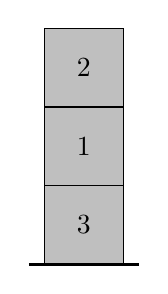
\begin{tikzpicture}
    \draw[fill=lightgray] (0,0) rectangle (1,1) rectangle (0,2)rectangle (1,3);
    \draw[thick] (-.2,0)--(1.2,0);
    \node (A) at (.5,.5) {3};
    \node (B) at (.5,1.5) {1};
    \node (C) at (.5,2.5) {2};
\end{tikzpicture}
\end{center}

On considère la fonction suivante:

\begin{pythoncode}
def mystere(pile1, pile2):
    if est_vide(pile1):
        return pile2
    else:
        empiler(pile2, depiler(pile1))       
        return mystere(pile1, pile2)
    \end{pythoncode}



\textbf{1.} Dans cette question on a \pythoninline{p = 30 : 20 : 10} et \pythoninline{q = 40 : 50 : 60}. Que renvoie l' appel \pythoninline{mystere(p,q)} ?
\begin{encadre}[Réponse]
Il renvoie \pythoninline{10 : 20 : 30 : 40 : 50 : 60}.
\end{encadre} 
\textbf{2.} Expliquer en une phrase la fonction \pythoninline{mystere}.
\begin{encadre}[Réponse]
Cette fonction dépile la première pile pour l'empiler sur la deuxième.
\end{encadre} 
\textbf{3.} Dans cette question on a \pythoninline{p = 10 : 20}.\\
    Que se passe t-il lors de l’appel mystere(p , p) ?
\begin{encadre}[Réponse]
À ce moment la fonction dépile et empile à nouveau indéfiniment la valeur 10 sur \pythoninline{p}, jusqu'à saturer la pile de récursion. 
\end{encadre} 


\exo\\


\'Ecrire en \textsc{Python} une fonction \pythoninline{max_file} qui
\begin{enumerate}[--]
    \item 	en entrée prend une file \textbf{non vide} composée d'\pythoninline{int} \textbf{positifs};
    \item 	renvoie le maximum de cette file. Attention la file doit être remise dans l'état initial et aucune autre structure de données (pile, file, liste) ne doit être utilisée.
\end{enumerate}

\begin{exemple}[ d'utilisation]
\begin{minted}{python}
>>> print(F)
>>> 2 -> 3 -> 5 -> 1
>>> max_file(F)
>>> 5
>>> print(F)
>>> 2 -> 3 -> 5 -> 1
\end{minted}
\end{exemple}
\begin{encadre}[Réponse]
\begin{minted}{python}
def max_queue(file):
    resultat = -1 # notre maximum temporaire
    enfiler(file, -1) # on enfile -1 pour savoir quand s'arrêter
    valeur = defiler(file)
    while valeur != -1:
        enfiler(file, valeur)
        if valeur > resultat:
            resultat = valeur
        valeur = defiler(file)
    return resultat
\end{minted}
\end{encadre}



\end{document}

\exo\\
\begin{enumerate}[\bfseries 1.]
    \item 	Écrire une fonction \textsc{Python} \pythoninline{est_dans_liste()} qui 
    \begin{enumerate}[--]
        \item 	en entrée prend une liste \pythoninline{lst} d'entiers et un entier \pythoninline{x};
        \item 	renvoie \pythoninline{True} si \pythoninline{x} est dans \pythoninline{lst} et \pythoninline{False} sinon.	
    \end{enumerate}
    \textbf{Attention : la recherche doit s'arrêter dès que \pythoninline{x} est trouvé et il est interdit d'utiliser \pythoninline{return x in lst}.}
    \item 	\pythoninline{tab} représente un \og tableau à deux dimensions\fg{}, implémenté sous forme de liste de listes.\\\
    Par exemple \pythoninline{tab = [[1, 3, 4], [5, 2, 1]]} permet de représenter le tableau 
    $$\begin{pmatrix}
        1 &3 & 4\\\
        5 &2 &1\\
    \end{pmatrix}$$
    Écrire une fonction \pythoninline{est_dans_tableau2D} qui 
    \begin{enumerate}[--]
        \item 	prend en entrée une liste de listes d'entier \pythoninline{tab} et un entier \pythoninline{x};
        \item 	renvoie \pythoninline{True} si \pythoninline{x} figure dans \pythoninline{tab} et \pythoninline{False} sinon.	
    \end{enumerate}
    \textbf{Attention : cette fonction doit utiliser la fonction \pythoninline{est_dans_liste}.}
    \item  Si \pythoninline{tab} est une liste de $n$ listes de longueur $p$, quelle est le nombre de tests qu'effectue \pythoninline{est_dans_tableau2D} dans le pire des cas ?
\end{enumerate}